\documentclass[10pt,a4paper]{article}
\usepackage[margin=2.2cm]{geometry}\usepackage{booktabs,graphicx,amsmath,hyperref,caption}
\title{Supply-Aware Sequential Matching: Round 2 Technical Report}
\author{Kashmira Matale (solo entry)}\date{17 October 2026}
\begin{document}\maketitle
\noindent\textbf{Challenge:} Vouchsafe $\times$ IITM, Sequential Matching Problem (kit 1.0.0). Synthetic simulator only; nothing here is evidence about real people. Primary outcome: msmi per 100 arrived members, reported with calibration and who is left waiting.

\section{Summary}
Round 2 asked three questions. (1) The stdlib build reproduces the Round~1 prototype's decisions and, within noise, its results. (2) Shrunk member propensities, with priors recalibrated on selection seeds, do not show a reliable gain over a constant prior on fresh seeds; their ranking signal is weak (AUC $0.55$, Brier equal to the base rate). (3) Under changed missingness and response behaviour, targeted constraint asks remain essential, soft-field asks never pay, and learning is at most weakly useful; the stress runs have only 4 episodes per condition, so this part is suggestive. The one change that held on both seed sets is a \emph{waiting priority}: it reduces members left waiting and waiting time without a detectable change in msmi, mutual acceptances or dates against the supplied greedy baseline. It does trade away the mutual-acceptance gain that the Round~1 build showed pooled.

\section{What changed}
\textbf{Round 2 default (\texttt{r2}).} Every member has the same prior (no learned propensities); the daily batch is an exact maximum-weight matching (components $\le18$ members, greedy beyond); an edge weight is multiplied by $1+\lambda(s_a+s_b)$ with $\lambda=2$, where $s_i=\min(\text{days since arrival},30)/30$ for members never yet introduced and $0$ otherwise; matching relationship\_goal (when both are observed) multiplies by 1.5; hard-constraint asks are targeted; no soft asks. \textbf{Round~1 build (\texttt{r1}):} learned Beta-shrunk propensities, no waiting term; kept as a profile. Hard eligibility always comes from the supplied \texttt{kit.eligibility}; outputs are re-validated and fall back to the supplied baseline on any error. The waiting term is my own definition; $\lambda$ was not tuned beyond a sweep.

\section{Protocol}
All comparisons are paired on identical worlds, in-process, with the unmodified simulator (an exact memo of \texttt{eligibility} only speeds it up). \emph{Stage A} (selection): seeds 3001--3009 $\times$ 6 scenarios $=54$ episodes. \emph{Stage C} (fresh, untouched during selection): seeds 6001--6006 $\times$ 6 $=36$. \emph{Stress}: seeds 7001--7004 in five modified worlds (70\% of answers removed and 15\% declined; response rates $\times0.6$; response rate halved at day 30; bimodal response rate; strong member acceptance bias), 20 episodes. Intervals are 95\% percentile bootstraps over paired episode differences (2000 resamples). ``Left waiting'' counts members with a truly feasible partner who never received an introduction; it uses simulator truth after the fact and is a diagnostic only. Calibrated priors were fitted by beta-binomial maximum likelihood on stage-A feedback only: responds $(0.78,12)$, Yes $(0.45,8)$, second-meeting Yes $(0.66,50\text{, capped})$ versus hand-set $(0.8,4),(0.4,4),(0.53,3)$.

\section{Results}
\begin{table}[h]\centering\small
\resizebox{\linewidth}{!}{\begin{tabular}{lrrrrr}\toprule
Policy (vs greedy) & Left waiting & Mean wait (d) & msmi/episode & Mutual acc. & Dates\\\midrule
Round 1 build & $-0.30$ [$-0.60,0.00$] & $-0.80$ [$-0.99,-0.60$] & $+0.11$ [$-0.16,+0.38$] & $+0.66$ [$+0.02,+1.31$] & $+0.61$ [$-0.10,+1.40$]\\
Constant prior, no waiting & $-0.23$ [$-0.58,+0.12$] & $-0.79$ [$-1.00,-0.59$] & $+0.11$ [$-0.12,+0.34$] & $0.00$ [$-0.74,+0.76$] & $-0.08$ [$-0.81,+0.77$]\\
\textbf{Round 2 (waiting)} & $-1.24$ [$-1.52,-0.96$] & $-1.00$ [$-1.18,-0.81$] & $+0.08$ [$-0.19,+0.37$] & $-0.07$ [$-0.77,+0.63$] & $-0.06$ [$-0.83,+0.76$]\\
Waiting + learned & $-1.27$ [$-1.54,-0.99$] & $-0.95$ [$-1.13,-0.77$] & $+0.21$ [$-0.06,+0.47$] & $+0.09$ [$-0.53,+0.71$] & $+0.22$ [$-0.51,+0.96$]\\
Waiting, greedy alloc. & $-1.14$ [$-1.42,-0.88$] & $-0.96$ [$-1.14,-0.79$] & $-0.07$ [$-0.27,+0.13$] & $-0.09$ [$-0.60,+0.44$] & $+0.31$ [$-0.27,+0.87$]\\
Waiting, baseline asks & $-1.00$ [$-1.27,-0.73$] & $-0.23$ [$-0.36,-0.10$] & $+0.14$ [$-0.03,+0.32$] & $+0.01$ [$-0.59,+0.60$] & $+0.08$ [$-0.50,+0.66$]\\
Waiting + soft asks & $-1.20$ [$-1.48,-0.92$] & $-1.02$ [$-1.21,-0.84$] & $+0.01$ [$-0.24,+0.30$] & $-0.32$ [$-1.04,+0.42$] & $-0.29$ [$-1.06,+0.53$]\\\bottomrule
\end{tabular}}
\caption{Pooled stages A+C (90 paired episodes), difference from the supplied greedy baseline. Ask cost: $-3$ units for targeted asks, $0$ for baseline asks, $+51.5$ for soft asks. Greedy's mean is about 0.7 msmi per episode.}\end{table}

\paragraph{Q1: does the build reproduce the prototype?} On fresh seeds the prototype (networkx blossom, soft asks) versus the stdlib Round~1 build differs by $-0.28$ msmi [$-0.69,+0.14$] and $+0.22$ mutual acceptances [$-0.44,+0.97$], within noise; it does spend $+53.7$ ask units and gets $+0.89$ dates [$+0.17,+1.67$] (one of eight outcomes, not corrected for multiplicity). At the decision level, on 337 days from 9 fresh episodes the exact stdlib matching has the same total weight as networkx on 333 days (98.8\%) and the identical pair set on 285 (84.6\%; ties). The largest value gap is 5.8\%, and exactly four days had a component above the 18-member exact limit, as many as the unequal days.

\paragraph{Q2: do calibrated propensities help?} Hand-set predictions of mutual acceptance average 0.10 against 0.137 observed; fitted priors give 0.118. On fresh seeds the Brier score is 0.119 (hand-set) and 0.118 (fitted), identical to predicting the base rate (0.118); AUC is 0.554 and 0.549 (0.52 on stage A). Fitted-prior versus constant-prior outcomes on fresh seeds: msmi $+0.08$ [$-0.17,+0.31$], mutual acceptances $+0.56$ [$-0.14,+1.28$]. Hand-set learned versus constant prior, pooled: msmi $+0.13$ [$+0.02,+0.26$], mutual acceptances $+0.16$ [$-0.28,+0.59$], but fresh seeds alone gave $+0.17$ [$-0.06,+0.42$] msmi and the best-looking variant was chosen among many, so I do not call it confirmed. An oracle using the simulator's true acceptance probabilities gets $+1.03$ mutual acceptances [$+0.25,+1.81$] over greedy on fresh seeds but no gain on waiting, so ordering signal exists but is small relative to what 1--3 observations per member can learn.

\paragraph{Q3: changing conditions.} With only 4 episodes per condition, intervals are wide. Pooled over the 20 stress episodes the waiting rule still lowers members left waiting ($-0.30$ [$-0.55,-0.05]$ vs greedy), and targeted constraint asks remain essential: removing all asks adds $+37.9$ [$+30.7,+44.4$] left-waiting members and loses 5.0 mutual acceptances versus greedy. Soft asks cost about $+45$ units for $+0.05$ msmi [$0.00,+0.15$] over the default and never helped. Learning on top of the default is $+0.05$ msmi [$-0.10,+0.20$] overall and $+0.25$ [$0.00,+0.75$] in each of the two conditions where members really differ (bimodal response, strong acceptance bias), the only place a gain is plausible; when response behaviour drops mid-episode it is $-0.25$ [$-0.75,0.00$]. Baseline asks give $+0.65$ mutual acceptances versus the default for $+2.6$ units, again within noise. The 70\%-missing world is degenerate (greedy coverage 0.04).

\begin{figure}[h]\centering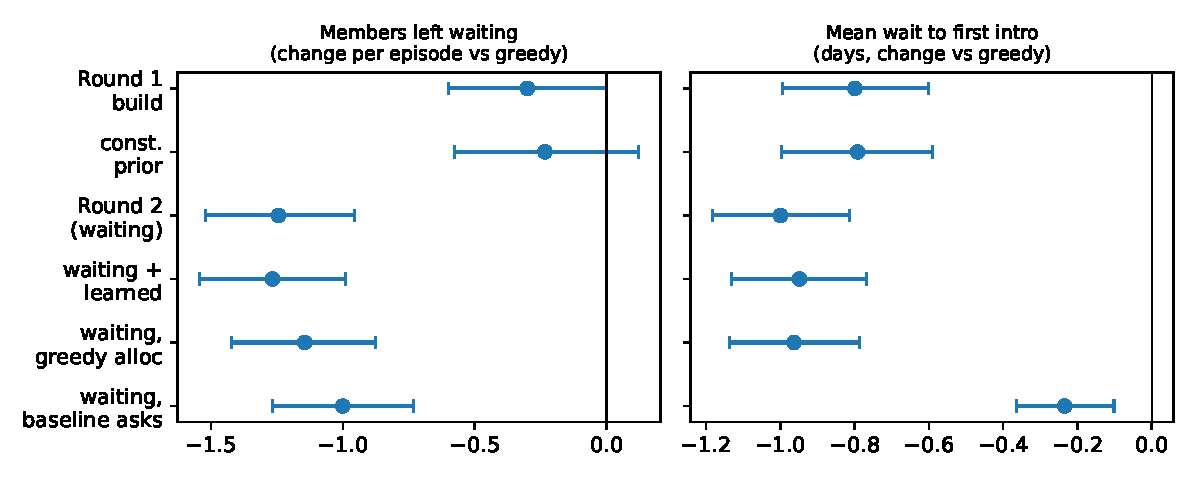
\includegraphics[width=.72\linewidth]{results/fig_waiting.pdf}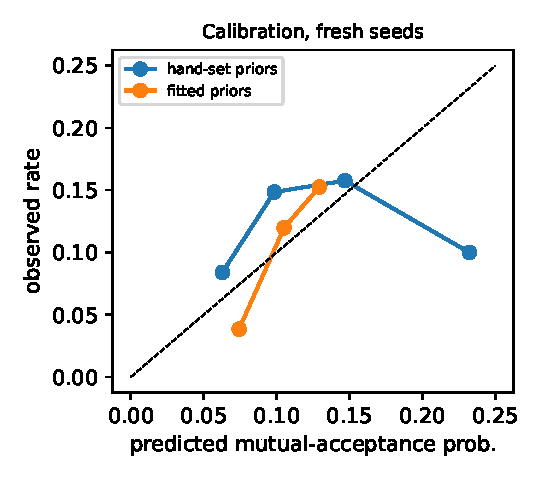
\includegraphics[width=.26\linewidth]{results/fig_calibration.pdf}\caption{Left: paired differences from greedy (pooled A+C, 95\% intervals). Right: reliability of the mutual-acceptance prediction on fresh seeds.}\end{figure}

\section{What the comparisons taught}
(i) The waiting priority does the work: exact matching adds nothing over greedy allocation with the same priority on who is left waiting ($-1.24$ vs $-1.14$), so a simpler allocator would do; I keep exact matching because it costs 0.13\,s per call. (ii) Against the Round~1 build, the waiting rule is a trade: pooled, Round~1 has $+0.72$ [$+0.23,+1.20$] mutual acceptances and $+0.67$ [$+0.20,+1.16$] dates over Round~2 but leaves $0.94$ [$0.67,1.23$] more members waiting; Round 2 is only ``free'' relative to greedy. (iii) The waiting+learned variant recovers most of both but did not beat the default on fresh seeds alone; it is the candidate for a properly powered Round~3. (iv) Targeted asks are mainly a waiting-time tool (mean wait $-1.00$ vs $-0.23$ with baseline asks), not a cost saver ($-3$ units). (v) msmi stays too rare (under one event per episode) to separate any of these; mutual acceptance, dates and waiting are the usable outcomes.

\section{Limitations}
Stage-A selection used about eleven policies, so its single positive msmi results are subject to selection; stage C and the pooled intervals are uncorrected for multiplicity. Stress runs have 4 episodes per condition. $\lambda=2$ is an untuned choice (1, 2, 4 gave the same left-waiting result on stage A). The official evaluator was run for seed 101 only (all six scenarios valid; primary score 0.50, coverage 0.4175, mutual acceptances 8.5 per 100, ask cost 199, 8.3 s inference in total); the Docker container build was not run in my environment.

\section{Reproducibility and provenance}
Python 3.12, standard library only for the policy; analysis used numpy, scipy, matplotlib and networkx (prototype only). No training; priors fixed constants or fitted on seeds 3001--3009; deterministic. See \texttt{README\_SUBMISSION.md} and \texttt{run\_round2.sh}. The simulator source was read to design experiments and the oracle uses simulator truth only inside the evaluation harness. Coding and analysis assistance: Claude (Anthropic); every reported number comes from the included result files.
\end{document}
